\section{Tổng kết}
Trong chương này, chúng ta đã khám phá các khái niệm và phương pháp để trực quan hóa dữ liệu chuỗi thời gian. Chương này cũng đã trình bày cách sử dụng các đặc trưng của dữ liệu chuỗi thời gian trong các kỹ thuật trực quan hóa khác nhau. Các đặc trưng này bao gồm dữ liệu, thời gian và hình ảnh biểu diễn trực quan (xem Phần 3.1). Vì có thể quan sát được những điểm cân xứng và bất cân xứng liên quan đến cách phân loại của chúng tôi, do đó, độc giả nên dành thời gian để xem xét kỹ lưỡng những phần diễn giải cụ thể ở các nội dung đã trình bày.
\begin{itemize}
    \item \textit{Dữ liệu: hệ quy chiếu}. Trong khảo sát này [5], các tác giả chủ yếu tập trung vào loại dữ liệu trừu tượng. Việc biểu diễn dữ liệu chuỗi thời gian trong khung tham chiếu không gian đòi hỏi nhiều hơn đáng kể trong hoạt động thiết kế vì phải đóng gói nhiều thông tin hơn vào trong cùng một biểu đồ trực quan. Đặc biệt là khi đã có các ngành khoa học liên quan đến bản đồ học, vốn là những lĩnh vực nghiên cứu độc lập có lịch sử hình thành và phát triển lâu dài, đã phát triển các phương pháp tiếp cận để kết hợp trực quan hóa các khía cạnh thời gian và không gian của dữ liệu [16, 17, 256]. Hơn nữa, dữ liệu không gian nói chung và không gian địa lý nói riêng cũng đã được trình bày trong Chương 5 và 6.
    \item \textit{Thời gian: sắp xếp}. Hầu hết các kỹ thuật trong khảo sát của chúng tôi [5] tập trung vào việc biểu diễn thời gian theo trình tự tuyến tính; các cách tiếp cận với thời gian theo trình tự tuần hoàn được đề cập ít hơn tương đối. Lý do cho điều này có thể là do người dùng thường quan tâm đến các xu hướng phát triển từ quá khứ, đến hiện tại, đến tương lai hơn là tìm kiếm các chu kỳ tuần hoàn trong dữ liệu.
    \item \textit{Thời gian: nguyên thủy thời gian}. Thời điểm tức thời là nguyên thủy thời gian được sử dụng phổ biến nhất trong khảo sát của chúng tôi [5]. Điều này có vẻ hoàn toàn tự nhiên bởi vì dữ liệu thường được đo lường tại một thời điểm cụ thể. Việc đo lường theo khoảng thời gian thường ít xảy ra hơn và chủ yếu là trong các trường hợp cần đến việc lập kế hoạch.
    \item \textit{Trực quan hóa: ánh xạ}. Rõ ràng, các kỹ thuật ánh xạ tĩnh thì thường phù hợp hơn để biểu diễn trên một trang sách thay vì ánh xạ động. Vì thế, các kỹ thuật trực quan hóa được chọn ở chương này có chút thiên lệch khi tập trung nhiều vào các phương pháp ánh xạ tĩnh. Tuy nhiên, các kỹ thuật ánh xạ động cũng vô cùng quan trọng và nó thường là giải pháp đầu tiên được đưa ra khi trực quan hóa dữ liệu chuỗi thời gian.
    \item \textit{Trực quan hóa: số chiều}. Các phương thức biểu diễn trực quan 2D thường được ưa chuộng hơn so với 3D, vì chúng thường khái quát hơn và do đó dễ hiểu hơn. Và vì thế, một lần nữa các kỹ thuật trực quan hóa đã được giới thiệu trong chương này chủ yếu thiên về phương pháp tiếp cận 2D. Đặc biệt là các kỹ thuật sơ khai có xu hướng gắn liền với không gian hai chiều đơn giản do khả năng tính toán hạn chế khi đó. Tuy nhiên, các công nghệ hiện đại đã giúp các nhà thiết kế trực quan hóa dễ dàng triển khai trực quan hóa 3D hơn và giúp điều hướng góc nhìn của người dùng khi khám phá các không gian thực tế ảo ba chiều. Điều này đặc biệt hữu ích khi trực quan hóa dữ liệu có tham chiếu không gian.
    \item \textit{Trình duyệt TimeViz}. Chúng tôi đã xây dựng một kho lưu trữ (http://survey. timeviz.net) giúp tìm kiếm các phương pháp có sẵn phù hợp với cách thức phân loại đã được giải thích trong Phần \ref{sub:3.1.cate} (xem Hình (\ref{fig:f7.17})). Việc tìm kiếm được thực hiện đơn giản thông qua việc lựa chọn các đặc trưng về thời gian, dữ liệu và biểu diễn trực quan, từ đó các kỹ thuật trực quan hóa phù hợp sẽ được đề xuất dựa trên các đặc trưng đã chọn. Việc cấu trúc kho của chúng tôi trên cơ sở từng trang (per-page) cho phép truy cập dễ dàng khi cần tham khảo nhanh một kỹ thuật cụ thể. Mỗi trang mô tả ngắn gọn bối cảnh, giải thích ý tưởng và các khái niệm chính, đồng thời chỉ ra ứng dụng của một kỹ thuật cụ thể. Phần mô tả chi tiết cũng giới thiệu tham chiếu đến các tài liệu gốc hoặc danh sách các tài liệu tham khảo trong trường hợp có nhiều ấn phẩm cần tham chiếu hoặc nhiều ấn phẩm khác nhau sử dụng cùng một phương pháp. Có thể nói Trình duyệt TimeViz là một công cụ tuyệt vời để tìm kiếm các kỹ thuật trực quan phù hợp theo ba khía cạnh đã nêu trên.
\end{itemize}
\begin{figure}[H] % places figure environment here   
    \centering % Centers Graphic
    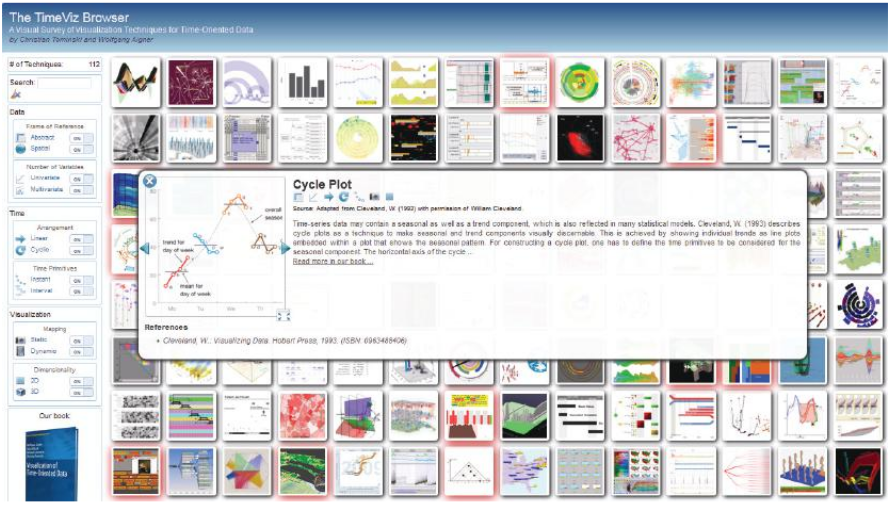
\includegraphics[width=1\textwidth]{assets/fig_7_17.png} 
    \caption{Trình duyệt TimeViz. Kho lưu trữ các kỹ thuật trực quan hóa cho dữ liệu chuỗi thời gian (http://survey.timeviz.net) [5].} % Creates caption underneath graph
    \label{fig:f7.17}
\end{figure}
